\section{Research as evidence acquisition and revision}\label{sec:C24:research}
A research workflow contains query construction, source acquisition, identity resolution, claim extraction, comparison, synthesis, and revision. Each stage can fail independently. A source can be relevant but outdated, a claim can be extracted accurately but applied to the wrong population, or a synthesis can cite a paper that never measured the asserted outcome. Counting citations or generated pages does not distinguish these errors.

Represent a claim as a tuple containing proposition, scope, evidence class, source version, result location, assumptions, and unresolved limitations. An evidence graph links claims to supporting or contradicting observations. This representation makes revision possible: if a paper changes its result, the system can identify dependent conclusions rather than rewrite every paragraph blindly. It also separates author-reported evidence from independent reproduction and analytical deduction.

The query policy should seek disconfirming evidence as well as support. A system rewarded for completing a coherent report can stop after finding sources that fit its initial hypothesis. A better evaluation includes questions where the decisive result is negative, where two studies use incompatible definitions, or where the available implementation cannot substantiate a headline claim. The correct output may be a narrower conclusion or an explicit unresolved state rather than a more confident answer.

Hosted research products and inspectable research harnesses occupy different reproducibility boundaries. DeerFlow exposes a research-oriented harness, while Asta's public resources distinguish research implementations from the hosted service~\cite{executionproduct029,executionproduct058}. Consequently, a result obtained with a published baseline cannot be attributed to every hosted variant, and a hosted demonstration does not reproduce the baseline. Evaluation must name the actual execution path and available tools.

The stopping condition is evidence sufficiency under a declared question, not exhaustion of a token budget or attainment of a target report length. An implementation can maintain unresolved claim categories and a bounded search frontier. It should report whether searches failed because no qualifying evidence was found, because a source was inaccessible, or because the budget ended. These states have different scientific implications and should not collapse into a single statement that evidence is absent.

\subsection{Biological agents: executable methods and empirical feedback}\label{sec:C24:biology}
The October 2026 biological frontier spans several distinct control loops. Paper2Agent converts papers and associated code into MCP interfaces and checks their executable behavior; its September Nature article demonstrates genomic and transcriptomic cases while retaining human responsibility for open-ended interpretation~\cite{miao2026paper2agent}. WetRobo's September report instead studies coding-agent adaptation of a laboratory robot kit on three equipment-manipulation tasks, including bottle-cap transfer between two laboratories~\cite{oikawa2026wetrobo}. Neither result alone establishes autonomous experimental discovery: method execution, equipment manipulation, scientific interpretation and selection of new experiments are different tasks with different ground truth.

This distinction determines what memory should retain. Reusing a numerical analysis method requires its data schema, software revision and assumptions. Reusing an equipment procedure additionally requires calibration, object geometry, admissible operating conditions and an execution monitor. Reusing a scientific conclusion requires evidence about the sampled biological system and measurement process. A skill that retains only successful command text can erase all three applicability boundaries. Model improvement does not repair a missing calibration record or turn an association into a validated mechanism.

The inspected Paper2Agent revision makes a limited verification boundary concrete. Its \path{validate_cases} routine can require positive acceptance cases for every expected tool; \path{check_subset} compares returned structures with declared expected values; \path{check_artifacts} checks returned artifact paths and identity conditions. Those functions support interface and smoke-case checks, not independent validation of a biological interpretation. The source was inspected at revision \texttt{8c2d059165ef}; no scientific analysis was executed here~\cite{paper2agent2026code}. Generated tests inherit the assumptions of their expected outputs. An executable wrapper can therefore improve method accessibility while faithfully automating an invalid analysis; interface conformance and scientific validity must remain separate claims.

Figure~\ref{fig:C24:scientificloop} locates the evidence and execution boundaries in a conceptual scientific-agent loop.
\begin{figure}[!htbp]
\centering
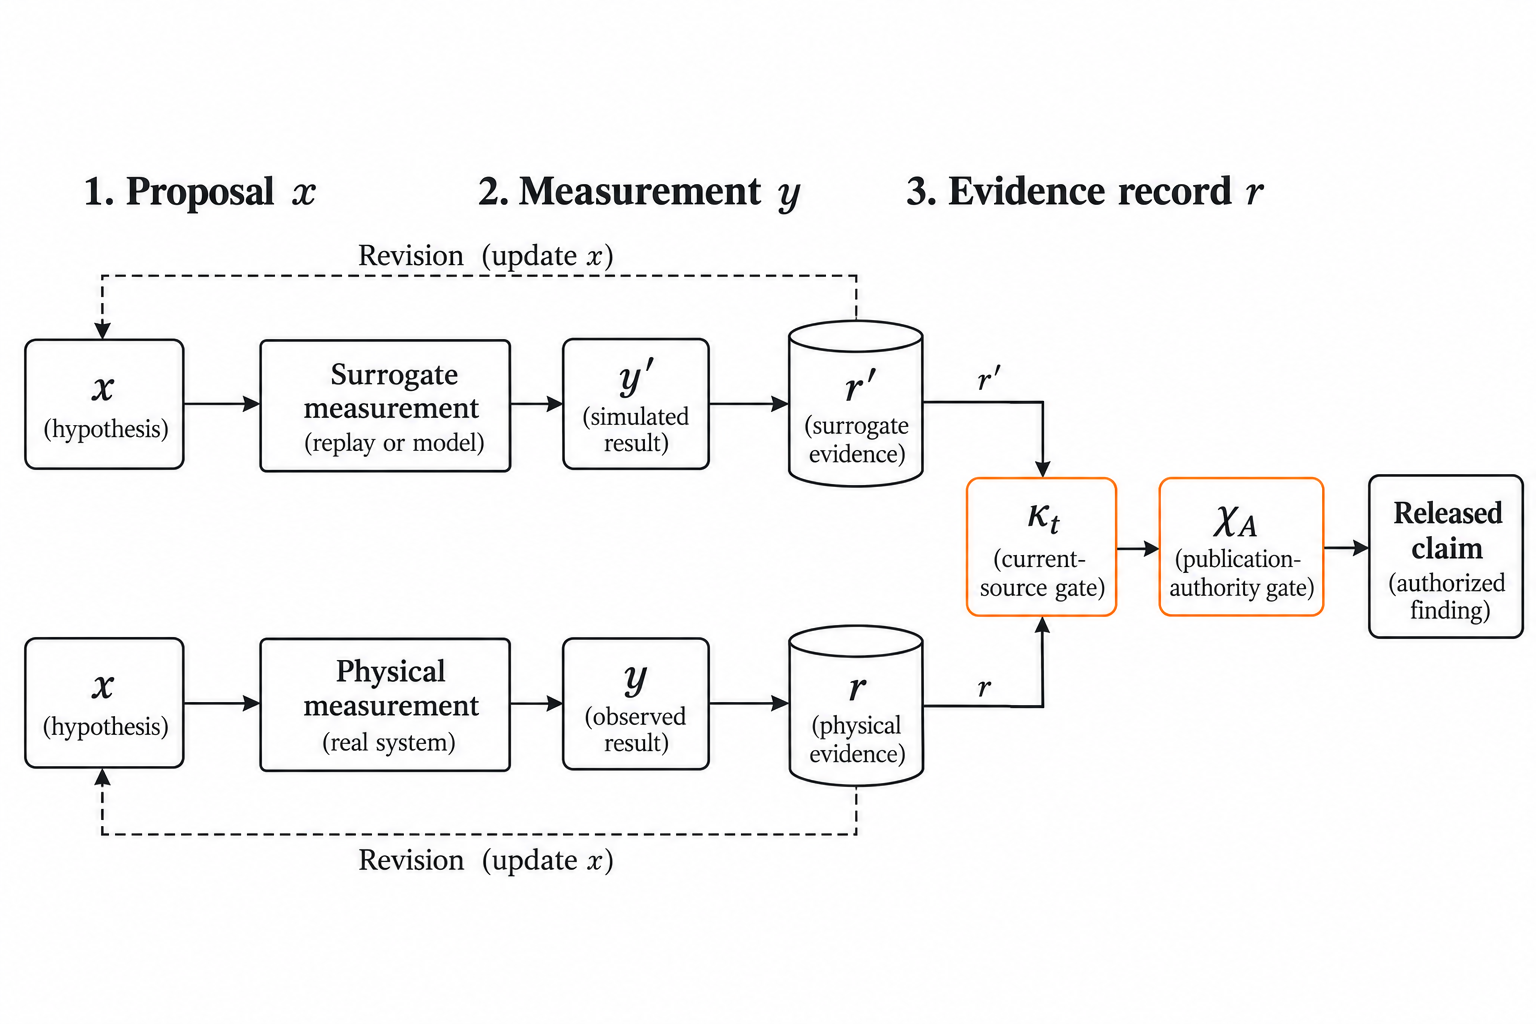
\includegraphics[width=\linewidth]{book/figures/assets/F24review.png}
\caption{Only records already accepted by the declared verifier enter the current-source validity and publication-authority gates. A released surrogate or replay finding retains its backend and recording provenance; it is not fresh physical evidence. Closing either loop does not identify a causal improvement or establish unrestricted laboratory autonomy.}
\label{fig:C24:scientificloop}
\end{figure}

\subsection{An October closed-loop result and its attribution limits}
Cutts and colleagues report three agent-guided aptamer design--test--improve rounds in October 2026~\cite{cutts2026aptamers}. The myoglobin results in Table~\ref{tab:C24:aptamers} are nonmonotonic across rounds. Human researchers performed the laboratory workflow, and the agent platform changed after the first round. The study therefore provides empirical evidence of iterative laboratory feedback and failure diagnosis, while its authors explicitly reserve matched-budget no-feedback and non-reasoning controls for future work. These observations do not isolate the causal contribution of agentic reasoning from harness changes, prior-round seeds or accumulated assay information.

\begingroup\setlength{\tabcolsep}{4pt}\small
\begin{table}[!htbp]
\centering
\caption{Author-reported bead-corrected myoglobin hits among newly designed primary candidates. Candidate populations differ across rounds; these are campaign observations, not randomized treatment-effect estimates. Source: Results R.2 of Cutts et al.~\cite{cutts2026aptamers}.}
\label{tab:C24:aptamers}
\begin{tabular}{lrrr}
\toprule Round & Hits & Candidates & Hit rate (\%) \\
\midrule
1 & 20 & 196 & 10.2 \\
2 & 9 & 244 & 3.7 \\
3 & 184 & 549 & 33.5 \\
\bottomrule
\end{tabular}
\end{table}
\endgroup

The nonmonotonic middle round is analytically important. Optimizing an assay proxy can concentrate candidates in a region with favorable background interactions rather than the desired biological property. A memory writer that records only the apparent successful motif can promote the shortcut into a procedural prior. A writer that retains target and background evidence, candidate lineage, analysis revision and uncertainty makes the lesson revisable. This is the biological counterpart of a coding agent memorizing a test-specific patch: a higher proxy score can accompany weaker alignment with the actual objective.

For a transparent analysis, consider the illustrative measurement model
\begin{align}
 y_{rk}&=f(x_{rk},e_r)+b_{p(r,k)}+\varepsilon_{rk},\\
 \mathbb E[\varepsilon_{rk}\mid x_{rk},e_r,p(r,k)]&=0.
\end{align}
Here $x_{rk}$ is candidate $k$ in round $r$, $e_r$ the declared assay conditions, $p(r,k)$ its measurement batch, $b_p$ a batch effect, and $y_{rk}$ the observed scalar response; all additive terms have the response's units. This is an analytical model, not a fitted model of the cited experiment. If candidate strategy changes only between batches, differences in $f$ and $b_p$ are not separately identified without additional design or assumptions. Randomized allocation within batches, recurring controls, replicated candidates and independent confirmation can address different parts of that ambiguity. Repeated reads of one construct are measurement replication; they do not create independent evidence about unrelated molecular families.

An agent-design comparison must therefore randomize complete campaigns or sufficiently isolated candidate allocations, preserve assay conditions and measurement budgets, and predeclare which feedback is available before each proposal. Include conventional sequential-design and no-feedback controls, not only a weak language-model prompt. Hold out candidate families or experimental regimes when the claim concerns transfer. Evaluate the selected designs and the learned predictor separately: finding a promising candidate and predicting unseen candidates are different achievements. Costs include physical measurements, waiting, failed jobs, analyst review and computational selection. Token expenditure alone is an inadequate resource boundary when empirical feedback dominates elapsed time.

\subsection{Replay laboratories, digital twins and live measurements}
Autonomous Science Bench, released in October 2026, makes that discovery--learning distinction explicit through two acceptance gates~\cite{wen2026asbench}. Version 0.1 contains six campaigns: five return recorded measurements and one uses a hidden surrogate. A live backend and adaptive allocation scheduler are planned, rather than evaluated results in that release. The laboratory service owns the measurement ledger independently of the agent, and grading combines measured-design quality with prediction on held-out designs. These design choices support controlled evaluation of sequential decisions; they do not constitute six live autonomous laboratory demonstrations.

The backend is part of the scientific claim. A replay can provide genuine historical measurements while excluding unrecorded designs. A digital twin permits more queries but tests optimization against its approximation and training coverage. A live assay adds drift, failed measurements, delayed returns and limits on reversibility. An interface that makes those backends look identical to the agent does not make their evidence interchangeable. Report backend provenance with every outcome and measure whether an agent exploits surrogate artifacts that fail under independent measurement.

Biological scope also constrains the autonomy claim. The aptamer study uses non-infectious protein targets under its stated laboratory conditions and does not study clinical efficacy, human subjects, or animal models~\cite{cutts2026aptamers}. An assay hit therefore remains an assay-specific observation. Extending a workflow to a different biological system requires its own material, measurement, containment, and approval conditions; preserving an API schema supplies none of those premises. The relevant system boundary includes the people or equipment that accept a proposed experiment and the independent evidence required before a scientific conclusion is promoted.

Delayed results create a further state boundary. Submitted, measured, quality-controlled and scientifically accepted experiments should have distinct identifiers and statuses. An agent must not treat an unreturned measurement as a negative label or spend the same physical budget twice after a timeout. When a result is corrected, dependent hypotheses and skills become stale without erasing the historical reason for their adoption. These requirements connect biological research to the session journal of Chapter~\ref{ch:C13}, the conditioning analysis of Chapter~\ref{ch:C17} and the recovery contracts of Chapter~\ref{ch:C32}. The cross-domain synthesis concerns preservation of evidence, authority and effect identity; it does not imply that software verifiers and biological assays have equivalent error models.
